\documentclass[a4paper, 14pt]{extarticle}

% Поля
%--------------------------------------
\usepackage{geometry}
\geometry{a4paper,tmargin=2cm,bmargin=2cm,lmargin=3cm,rmargin=1cm}
%--------------------------------------


%Russian-specific packages
%--------------------------------------
\usepackage[T2A]{fontenc}
\usepackage[utf8]{inputenc}
\usepackage[english, main=russian]{babel}

%--------------------------------------

\usepackage{textcomp}

% Красная строка
%--------------------------------------
\usepackage{indentfirst}               
%--------------------------------------             


%Graphics
%--------------------------------------
\usepackage{graphicx}
\graphicspath{ {./images/} }
\usepackage{float}%"Плавающие" картинки
%--------------------------------------

% Полуторный интервал
%--------------------------------------
\linespread{1.3}                    
%--------------------------------------

%Выравнивание и переносы
%--------------------------------------
% Избавляемся от переполнений
\sloppy
% Запрещаем разрыв страницы после первой строки абзаца
\clubpenalty=10000
% Запрещаем разрыв страницы после последней строки абзаца
\widowpenalty=10000
%--------------------------------------

%Списки
\usepackage{enumitem}

%Подписи
\usepackage{caption} 

%Гиперссылки
% \usepackage{hyperref}

\usepackage[colorlinks, urlcolor = blue, filecolor = blue, citecolor = blue, linkcolor = black]{hyperref}


\hypersetup {
unicode=true
}

%Рисунки
%--------------------------------------
\DeclareCaptionLabelSeparator*{emdash}{~--- }
\captionsetup[figure]{labelsep=emdash,font=onehalfspacing,position=bottom}
%--------------------------------------

\usepackage{tempora}

%Листинги
%--------------------------------------
\usepackage{listings} % Пакет для отображения кода
\usepackage{xcolor} % Пакет для цветных элементов

\lstset{inputencoding=utf8, extendedchars=false, keepspaces = true}

\definecolor{codegreen}{rgb}{0,0.6,0}
\definecolor{codegray}{rgb}{0.5,0.5,0.5}
\definecolor{codepurple}{rgb}{0.68,0.8,0.82}
\definecolor{backcolour}{rgb}{0.9,0.9,0.9} 
\definecolor{keyword}{rgb}{0.93, 0.68, 0.18}   % Оранжевые ключевые слова

\lstdefinestyle{mystyle}{
    backgroundcolor=\color{backcolour},   % цвет фона
    commentstyle=\color{codegreen},       % цвет комментариев
    keywordstyle=\color{keyword},        % цвет ключевых слов
    numberstyle=\tiny\color{codegray},    % стиль нумерации строк
    stringstyle=\color{codegreen},       % цвет строк
    basicstyle=\ttfamily\footnotesize,    % основной стиль текста
    breakatwhitespace=false,              % перенос по пробелам
    breaklines=true,                      % автоматический перенос строк
    captionpos=b,                         % позиция заголовка внизу
    keepspaces=true,                      % сохранять пробелы
    numbers=left,                         % нумерация строк слева
    numbersep=5pt,                        % отступ нумерации
    showspaces=false,                     % скрывать пробелы
    showstringspaces=false,               % скрывать пробелы в строках
    showtabs=false,                       % скрывать табуляцию
    tabsize=2                             % размер табуляции
}

\lstset{style=mystyle, inputencoding=utf8}



%--------------------------------------

%%% Математические пакеты %%%
%--------------------------------------
\usepackage{amsthm,amsfonts,amsmath,amssymb,amscd}  % Математические дополнения от AMS
\usepackage{mathtools}                              % Добавляет окружение multlined
\usepackage[perpage]{footmisc}


% графики
\usepackage{booktabs}        % Пакет для улучшенных таблиц
\usepackage{pgfplots}        % Пакет для построения графиков
\pgfplotsset{compat=1.17}    % Установка совместимости

% Литература 

% переименовываем  список литературы в "список используемой литературы"
\addto\captionsrussian{\def\refname{Список литературы}}






%--------------------------------------

%--------------------------------------
%			НАЧАЛО ДОКУМЕНТА
%--------------------------------------

\begin{document}

%--------------------------------------
%			ТИТУЛЬНЫЙ ЛИСТ
%--------------------------------------
\begin{titlepage}
\thispagestyle{empty}
\newpage


%Шапка титульного листа
%--------------------------------------
\vspace*{-60pt}
\hspace{-65pt}
\begin{minipage}{0.3\textwidth}
\hspace*{-20pt}\centering

\includegraphics[width=\textwidth]{emblem}
\end{minipage}
\begin{minipage}{0.67\textwidth}\small \textbf{
\vspace*{-0.7ex}
\hspace*{-6pt}\centerline{Министерство науки и высшего образования Российской Федерации}
\vspace*{-0.7ex}
\centerline{Федеральное государственное автономное образовательное учреждение }
\vspace*{-0.7ex}
\centerline{высшего образования}
\vspace*{-0.7ex}
\centerline{<<Московский государственный технический университет}
\vspace*{-0.7ex}
\centerline{имени Н.Э. Баумана}
\vspace*{-0.7ex}
\centerline{(национальный исследовательский университет)>>}
\vspace*{-0.7ex}
\centerline{(МГТУ им. Н.Э. Баумана)}}
\end{minipage}
%--------------------------------------

%Полосы
%--------------------------------------
\vspace{-25pt}
\hspace{-35pt}\rule{\textwidth}{2.3pt}

\vspace*{-20.3pt}
\hspace{-35pt}\rule{\textwidth}{0.4pt}
%--------------------------------------

\vspace{1.5ex}
\hspace{-35pt} \noindent \small ФАКУЛЬТЕТ\hspace{80pt} <<Информатика и системы управления>>

\vspace*{-16pt}
\hspace{47pt}\rule{0.83\textwidth}{0.4pt}

\vspace{0.5ex}
\hspace{-35pt} \noindent \small КАФЕДРА\hspace{50pt} <<Теоретическая информатика и компьютерные технологии>>

\vspace*{-16pt}
\hspace{30pt}\rule{0.866\textwidth}{0.4pt}

\vspace{11em}

\begin{center}
\Large {\bf Лабораторная работа №7} \\ 
\large {\bf по курсу <<Численные методы>>} \\
\large <<Тригонометрическая интерполиция функций
с помощью быстрого преобразования Фурье>> \\

\end{center}\normalsize

\vspace{8em}

\vbox{%
\hfill%
\vbox{%
\hbox{Студент:  }%
\hbox{Группа: ИУ9-61Б}%
\hbox{Преподаватель: Домрачева А.Б.}%
}%
} 

\bigskip

\vfill


\begin{center}
\textsl{Москва 2025}
\end{center}
\end{titlepage}
%--------------------------------------
%		КОНЕЦ ТИТУЛЬНОГО ЛИСТА
%--------------------------------------


\renewcommand{\ttdefault}{pcr}

\setlength{\tabcolsep}{3pt}


% Содержание:
%\tableofcontents
%\newpage

\newpage
\setcounter{page}{2}

\section{Постановка задачи}

\textbf{Дано:} Таблично заданная функция \( y_i = f(x_i) \) для \( i = 0, 1, \ldots, n \).
\begin{table}[H]
    \centering
    \begin{tabular}{|c|c|c|c|c|c|c|c|c|}
    \hline
    $x_i$ & 1.5 & 2.0 & 2.5 & 3.0 & 3.5 & 4.0 & 4.5 & 5.0 \\
    \hline
    $y_i$ & 0.16 & 0.68 & 1.96 & 2.79 & 3.80 & 6.81 & 9.50 & 24.86 \\
    \hline
    \end{tabular}
\end{table}

\textbf{Найти:}
\begin{enumerate}
    \item Выбрать вид аппроксимирующей функции из семейства двупараметрических моделей.
    \item Найти коэффициенты \( a \) и \( b \) методом наименьших квадратов.
    \item Вычислить среднеквадратичное отклонение.
\end{enumerate}

\section{Основные теоретические сведения}

\subsection{Аппроксимация двупараметрическими моделями}

Существует формальный подход для выбора вида аппроксимирующей функции, зависящей от двух параметров. Введем обозначения для средних значений:

\[
\begin{aligned}
x_a &= \frac{x_0 + x_n}{2} - \text{среднее арифметическое}, \\
x_g &= \sqrt{x_0 x_n} - \text{среднее геометрическое}, \\
x_h &= \frac{2}{\frac{1}{x_0} + \frac{1}{x_n}} - \text{среднее гармоническое}.
\end{aligned}
\]

Аналогично определяются \( y_a \), \( y_g \), \( y_h \) для значений функции. Рассматриваются девять функций с характеристическими свойствами:

\[
\begin{aligned}
z_1(x) &= ax + b \iff z(x_a) = y_a, \\
z_2(x) &= ax^b \iff z(x_g) = y_g, \\
z_3(x) &= ae^{bx} \iff z(x_a) = y_g, \\
z_4(x) &= a\ln x + b \iff z(x_g) = y_a, \\
z_5(x) &= \frac{a}{x} + b \iff z(x_h) = y_a, \\
z_6(x) &= \frac{1}{ax + b} \iff z(x_a) = y_h, \\
z_7(x) &= \frac{x}{ax + b} \iff z(x_h) = y_h, \\
z_8(x) &= ae^{b/x} \iff z(x_h) = y_g, \\
z_9(x) &= \frac{1}{a\ln x + b} \iff z(x_g) = y_h.
\end{aligned}
\]

\subsection{Алгоритм выбора функции}
\begin{enumerate}
    \item Построить график исходных данных и аппроксимирующей кривой.
    \item Вычислить \( x_a, x_g, x_h \) и \( y_a, y_g, y_h \).
    \item Определить \( z(x_a), z(x_g), z(x_h) \) по графику.
    \item Вычислить величины \( \delta_1, \ldots, \delta_9 \) и выбрать наименьшую.
\end{enumerate}

\section{Реализация}

\lstinputlisting[language=go, caption=lab6.py]{code/lab6.py}


\begin{figure}[H]
    \centering
    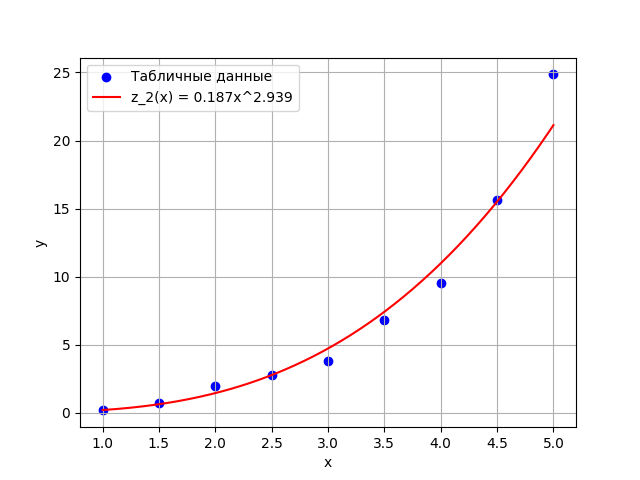
\includegraphics[width=0.8\textwidth]{images/graph.png}
    \caption{График исходных данных и аппроксимирующей функции $z_2(x) = 0.187x^{2.939}$}
    \label{fig:graph}
\end{figure}

Вычисленные значения:
\[
\begin{aligned}
x_a &= 3.000, \quad x_g = 2.236, \quad x_h = 1.667, \\
y_a &= 12.510, \quad y_g = 1.994, \quad y_h = 0.318, \\
z(x_a) &= 4.710, \quad z(x_g) = 1.986, \quad z(x_h) = 0.837.
\end{aligned}
\]

Вычисленные значения $\delta_i$:
\[
\begin{aligned}
\delta_1 &= |4.710 - 12.510| = 7.800, \\
\delta_2 &= |1.986 - 1.994| = 0.008, \\
\delta_3 &= |4.710 - 1.994| = 2.716, \\
\delta_4 &= |1.986 - 12.510| = 10.524, \\
\delta_5 &= |0.837 - 12.510| = 11.673, \\
\delta_6 &= |4.710 - 0.318| = 4.392, \\
\delta_7 &= |0.837 - 0.318| = 0.519, \\
\delta_8 &= |0.837 - 1.994| = 1.157, \\
\delta_9 &= |1.986 - 0.318| = 1.668.
\end{aligned}
\]

Наименьшее значение: \( \delta_2 = 0.008 \) (функция \( z_2(x) = ax^b \)).

Определение коэффициентов для функции \( z_2(x) = ax^b \):

Для функции \( z_2(x) = ax^b \) применяется следующая процедура:

1. Функция предварительно логарифмируется:
   \[
   \ln z_2(x) = \ln a + b \ln x
   \]

2. Минимизируется величина:
   \[
   \sum_{i=0}^{n} \left( \ln a + b \ln x_i - \ln y_i \right)^2
   \]

3. Решается система уравнений относительно \( \ln a \) и \( b \):
   \[
   \begin{cases}
   \ln a \cdot \sum (\ln x_i)^2 + b \cdot \sum \ln x_i = \sum (\ln x_i \ln y_i) \\
   \ln a \cdot \sum \ln x_i + b \cdot (n+1) = \sum \ln y_i
   \end{cases}
   \]

4. Элементы матрицы системы:
   \[
   \begin{aligned}
   A &= \sum (\ln x_i)^2 \\
   B &= \sum \ln x_i \\
   D_1 &= \sum (\ln x_i \ln y_i) \\
   D_2 &= \sum \ln y_i
   \end{aligned}
   \]

5. После решения системы по величине \(\ln a\) определяется коэффициент \(a\).

\section{Результаты}

\begin{table}[H]
    \centering
    \caption{Результаты аппроксимации}
    \begin{tabular}{lc}
    \toprule
    Параметр & Значение \\
    \midrule
    Выбранная функция & \( z_2(x) = ax^b \) \\
    Коэффициент \( a \) & 0.187 \\
    Коэффициент \( b \) & 2.939 \\
    Наименьшее значение \( \delta_2 \) & 0.008 \\
    Среднеквадратичное отклонение \( \Delta \) & 1.395722 \\
    \bottomrule
    \end{tabular}
\end{table}

\section{Вывод}

В ходе работы была выбрана аппроксимирующая функция \( z_2(x) = 0.187x^{2.939} \). Среднеквадратичное отклонение составило \( \Delta = 1.395722 \). Метод наименьших квадратов позволил точно определить коэффициенты функции, а характеристические свойства средних значений (арифметического, геометрического и гармонического) обеспечили корректный выбор модели.

\end{document}